\item Consider a unity feedback system as shown in the figure,shown with an integral compensator $\frac{k}{s}$ and open-loop transfer function
\begin{align}
 G(s) = \frac{1}{s^2+3s+2}
\end{align}   
   where $k>0$. Find the positive value of $k$ for which there are two poles of unity feedback system on the $\j\omega$ axis.
 \begin{figure}[!ht]
\centering
     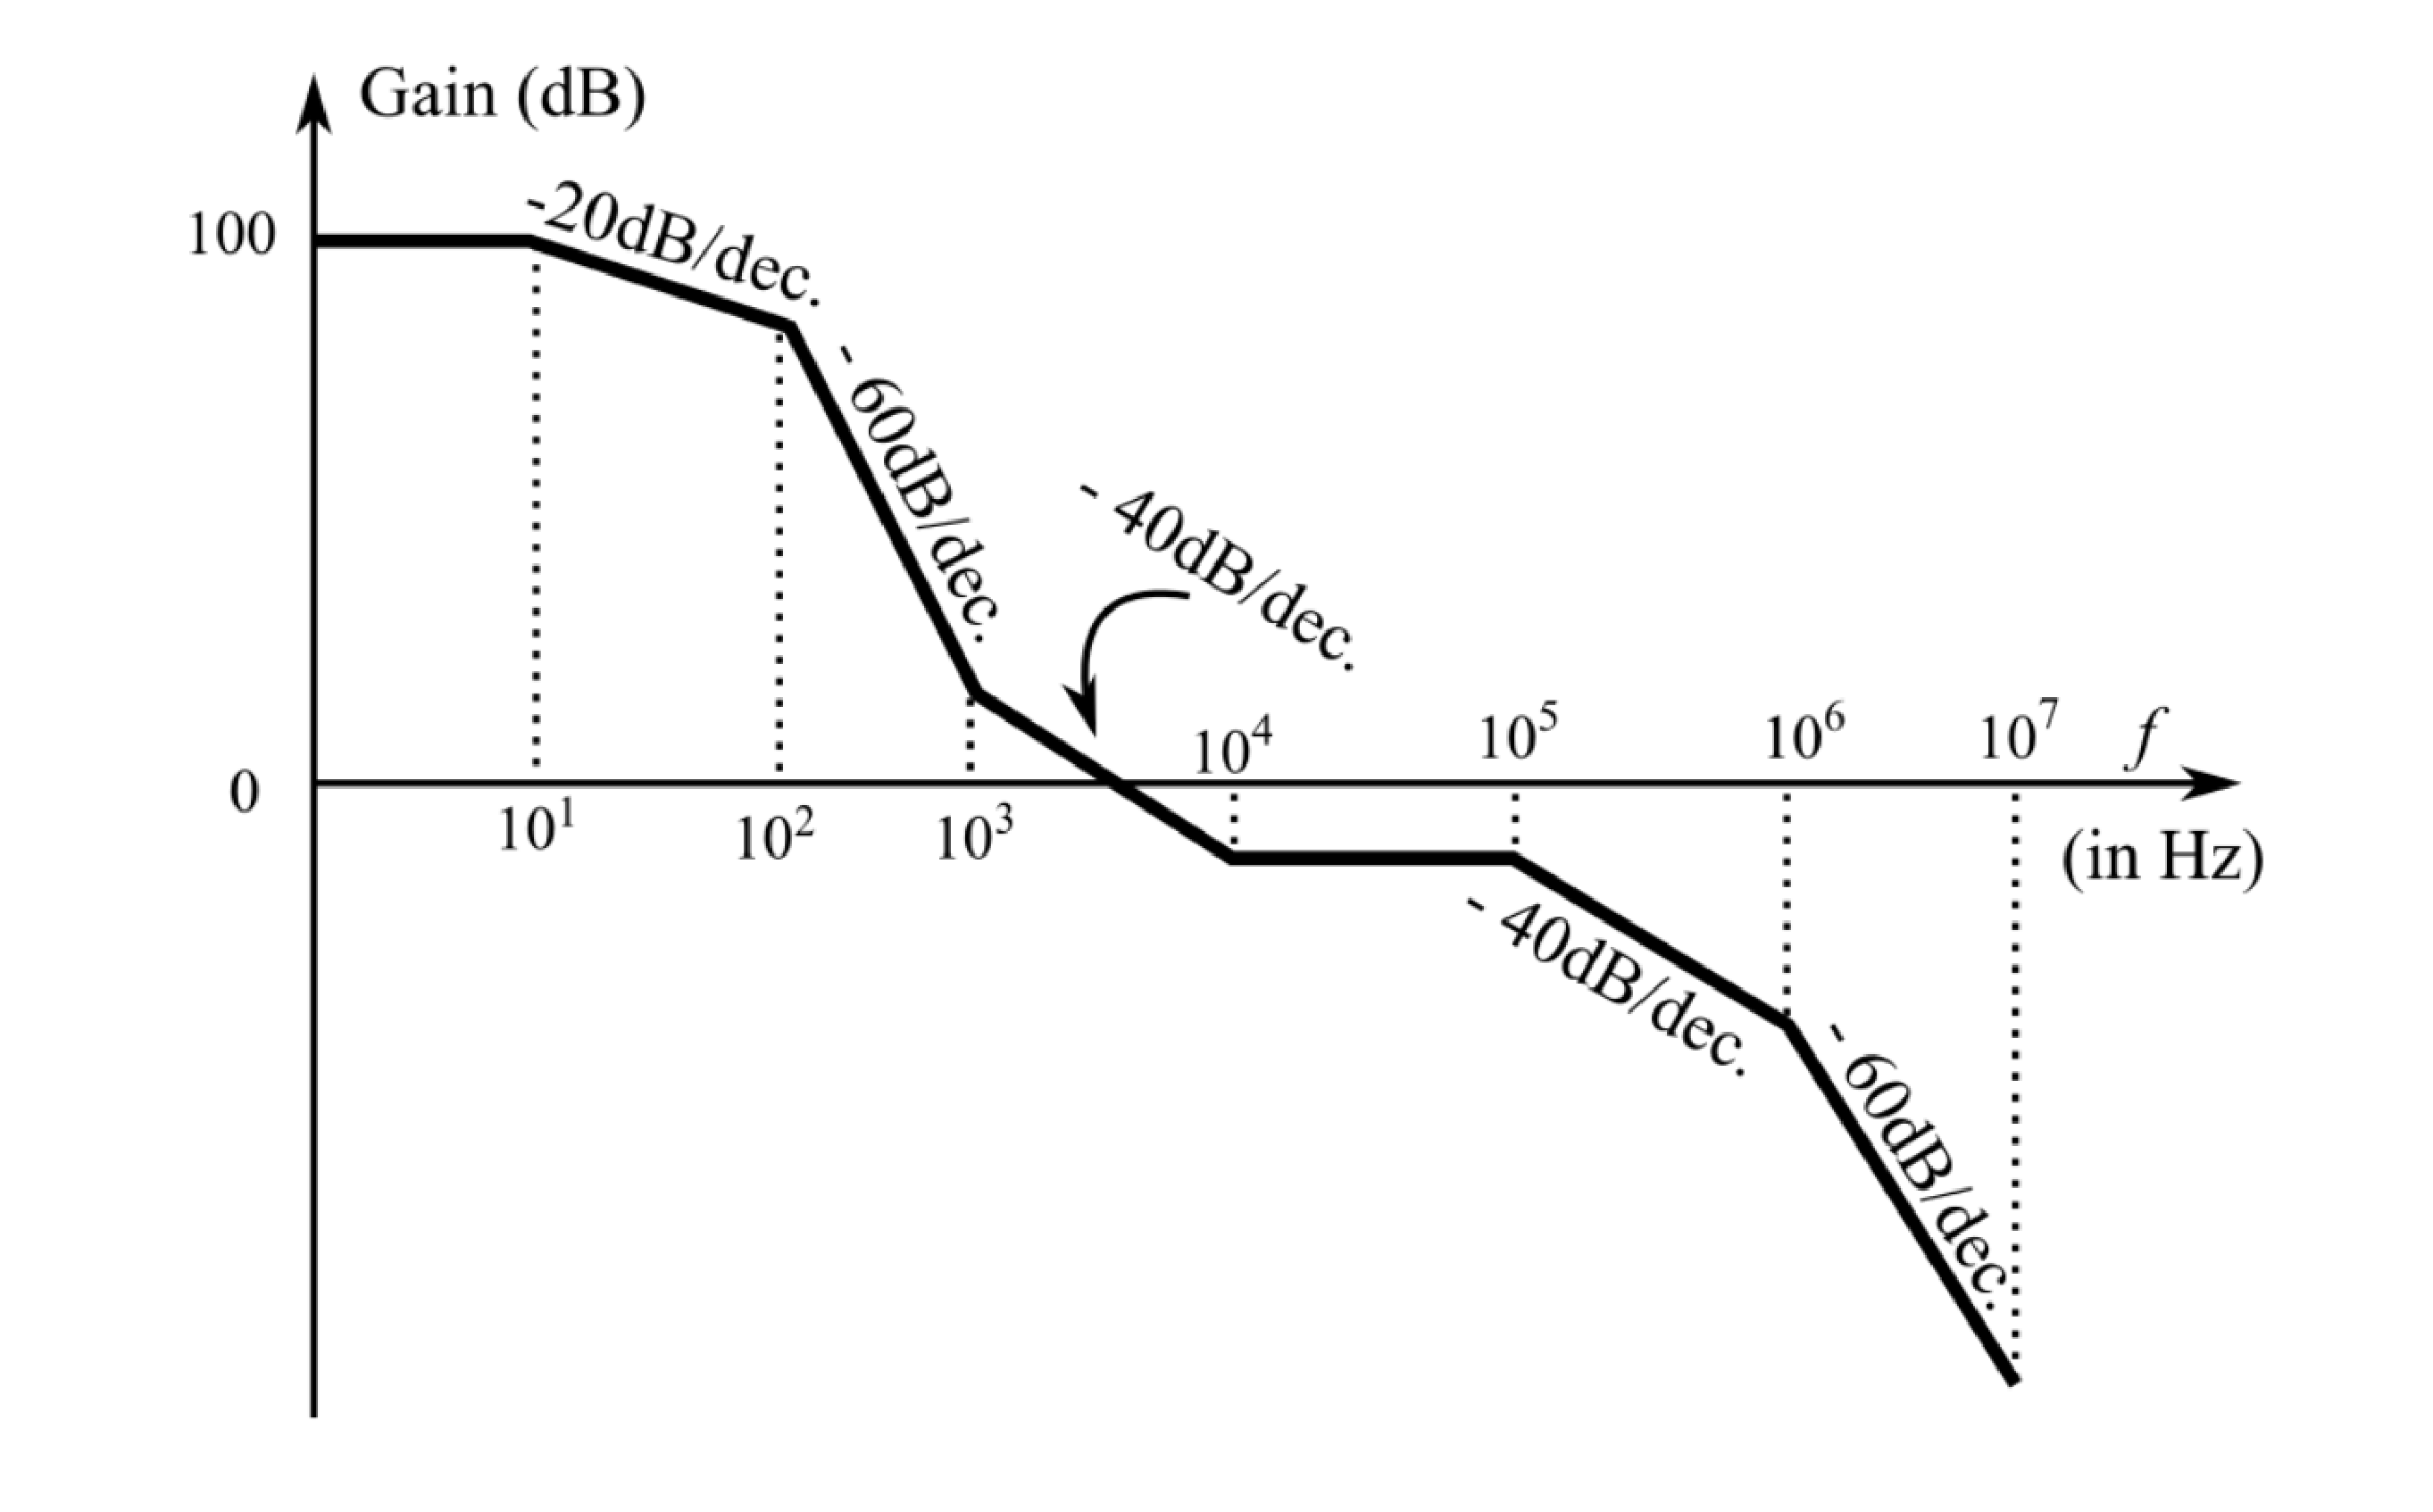
\includegraphics[width=\columnwidth]{./figs/ee18btech11001/ee18btech11001.eps}
\caption{}
\label{fig:routh}
    \end{figure}

\solution  The open loop transfer function
%
\begin{align}
G(s) = \frac{1}{s^2+3s+2}
\end{align}
%
Hence,
\begin{align}
H(s) = \frac{Y(s)}{X(s)} &= \frac{G(s)k/s}{1+G(s)k/s}
\\
&=  \frac{k}{1 + ks(s^2+3s+2)}
\end{align}
%
The poles of $H(s)$ are obtained from 
\begin{align}
s^3+3s^2+2s+k = 0
\end{align}
%
The corresponding Routh array is given by 
\begin{align}
\begin{vmatrix}
s^3\\s^2\\s^1 \\ s^0 
\end{vmatrix} 
\begin{vmatrix}
1 & 2 \\ 3 & k \\  \frac{6-k}{3} & 0\\ k & 0
\end{vmatrix}
\end{align}
%\newline $For poles on $j$\omega$ axis any one of the row should be zero
%\newline => $\frac{6-k}{3}$ = 0 or k = 0
%\newline But given k>0 ...
%\newline therefore, 6-k=0 => k = 6

